\section{Spiegazione del comportamento di condensatori in
	serie ed in parallelo. Determinazione della capacit\'a
	equivalente.}

Si definisce \textbf{Capacit\'a Equivalente} di una rete di condensatori la capacit\'a di un singolo condensatore che, sottoposto alla stessa differenza di potenziale $\Delta V$ a cui \`e soggetta la rete, assorbe la stessa corrente elettrica.

Nel caso di condensatori in serie avviene che, essendoci su tutto il ramo la stessa quantit\'a di carica :\\
\\
\noindent\begin{minipage}{0.3\textwidth}
$
\left\{
\begin{array}{llr}
	V_A - V_B = \frac{1}{C_1}Q_1 \\
	V_B - V_C = \frac{1}{C_2}Q_2 \\	
	V_A - V_C = \frac{1}{C_{eq}}Q_{eq} \\
	V_A - V_B + V_B - V_C = V_A - V_C  \\
	Q_1 = Q_2 = Q_{eq} = Q \\
	\\
	\textnormal{Passaggi Algebrici:}\\
	\frac{1}{C_1}\cancel{Q} + \frac{1}{C_2}\cancel{Q} = \frac{1}{C_{eq}}\cancel{Q} \\
	\frac{1}{C_1} + \frac{1}{C_2} = \frac{1}{C_{eq}}
\end{array}
\right.
$
\end{minipage}
\hfill%
\begin{minipage}{0.6\textwidth}\raggedleft
	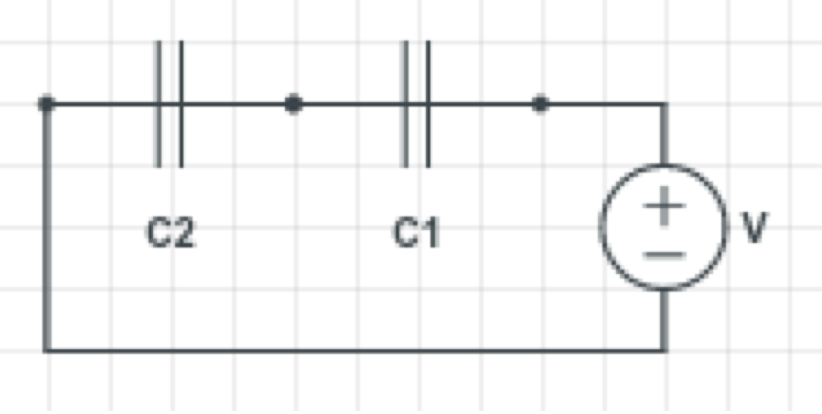
\includegraphics{serie_cond}
\end{minipage}
Pertanto la $C_{eq}$ vale $\frac{1}{C_1} + \frac{1}{C_2}$.\\
Nel caso di $n$ condensatori vale la seguente formula:
\begin{equation}
    C_{eq} = \sum{\frac{1}{C_i}}
\end{equation}
Dove tutte le $C_i$ sono in serie sullo stesso ramo.\\
\noindent\begin{minipage}{0.3\textwidth}
	$
	\left\{
	\begin{array}{lr}
	V_A - V_B = \frac{Q_1}{C_1} \rightarrow C_1 = \frac{Q_1}{V_A - V_B}   \\
	V_A - V_B = \frac{Q_2}{C_2}	\rightarrow C_2 = \frac{Q_2}{V_A - V_B}   \\
	V_A - V_B = \frac{Q_{eq}}{C_{eq}} \\
	Q_{eq} = Q_1 + Q_2\\
	\\
	\textnormal{Passaggi Algebrici:}\\
	V_A - V_B = \frac{Q_{eq}}{C_{eq}} = \frac{Q_1 + Q_2}{C_{eq}} = \\
	\frac{C_1(V_A - V_B) + C_2(V_A - V_B)}{C_{eq}} = \\
	\frac{(V_A - V_B)(C_1 + C_2)}{C_{eq}} \rightarrow \cancel{(V_A - V_B)} = \frac{\cancel{(V_A - V_B)}(C_1 + C_2)}{C_{eq}} \\
	C_{eq} = C_1 + C_2
	\end{array}
	\right.
	$
\end{minipage}
\hfill%
\begin{minipage}{0.6\textwidth}\raggedleft
	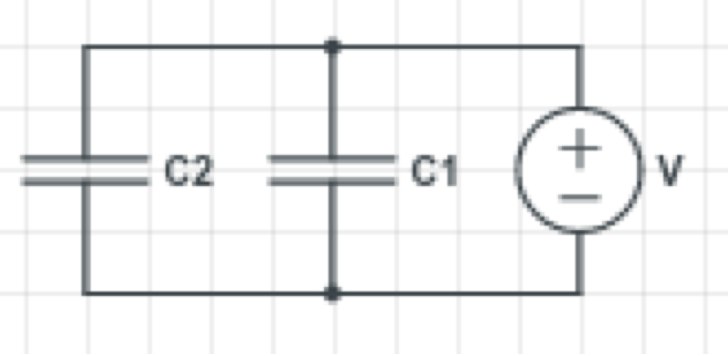
\includegraphics{parall_cond}
\end{minipage}
Pertanto la $C_{eq}$ vale $C_1 + C_2$.\\
Nel caso di $n$ resistori vale la seguente formula:
\begin{equation}
    R_{eq} = \sum{C_i}
\end{equation}
Dove tutte le $C_i$ sono in parallelo sullo stesso ramo.\\
\textbf{[Opzionale, dimostrare (11), (12), (13) e (14) per induzione su n]}
\begin{flushright}
	$\square$
\end{flushright}